% PenCast test deck: one slide per embed type the app must handle.
% Build: ./build.sh   (needs clip720p30.mp4 / clip1080p60.mp4 next to this file)
\documentclass[aspectratio=169]{beamer}
% noplaybutton: media9's play-button layer hides a `cm` in optional content, which
% Apple's PDF renderer skips, shifting everything after the video. See README.
\usepackage[noplaybutton]{media9}  % embedded video (RichMedia)
\usepackage{multimedia}  % \movie, linked video (Screen/Movie)
\usepackage{animate}     % frame animations
\usepackage{tikz}
\usepackage{pgfplots}
\pgfplotsset{compat=1.18}
\usetheme{Madrid}

\title{PenCast Test Deck}
\subtitle{media9 \textperiodcentered\ \textbackslash movie \textperiodcentered\ animate \textperiodcentered\ ink}
\date{}

\begin{document}

\begin{frame}
  \titlepage
\end{frame}

\begin{frame}[label=media9first]{1. media9: embedded MP4, autoplay + loop}
  \centering
  \includemedia[
    width=0.75\linewidth,height=0.421875\linewidth,
    activate=pageopen,
    addresource=clip720p30.mp4,
    flashvars={source=clip720p30.mp4&autoPlay=true&loop=true}
  ]{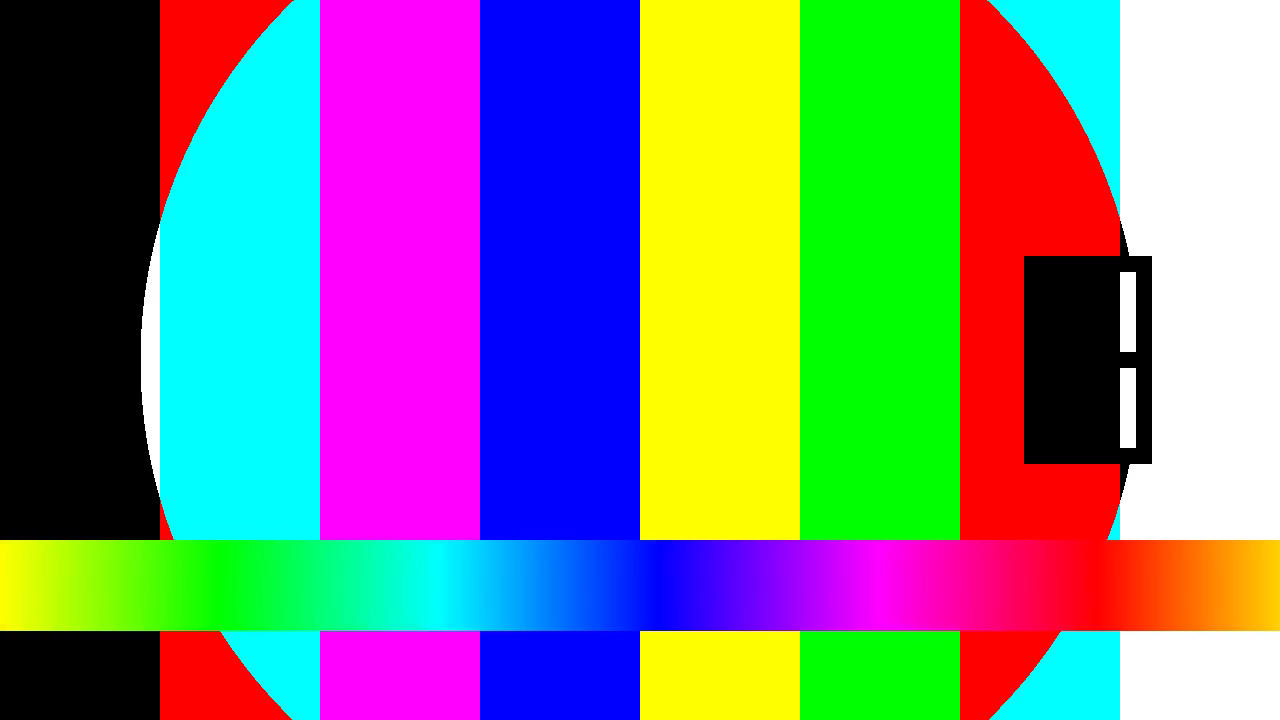
\includegraphics{poster720p30}}{VPlayer.swf}

  \small Draw over the playing video with the Pencil. Counter must not stutter.
\end{frame}

\begin{frame}{2. media9: 1080p60, click to play}
  \centering
  \includemedia[
    width=0.75\linewidth,height=0.421875\linewidth,
    activate=onclick,
    addresource=clip1080p60.mp4,
    flashvars={source=clip1080p60.mp4}
  ]{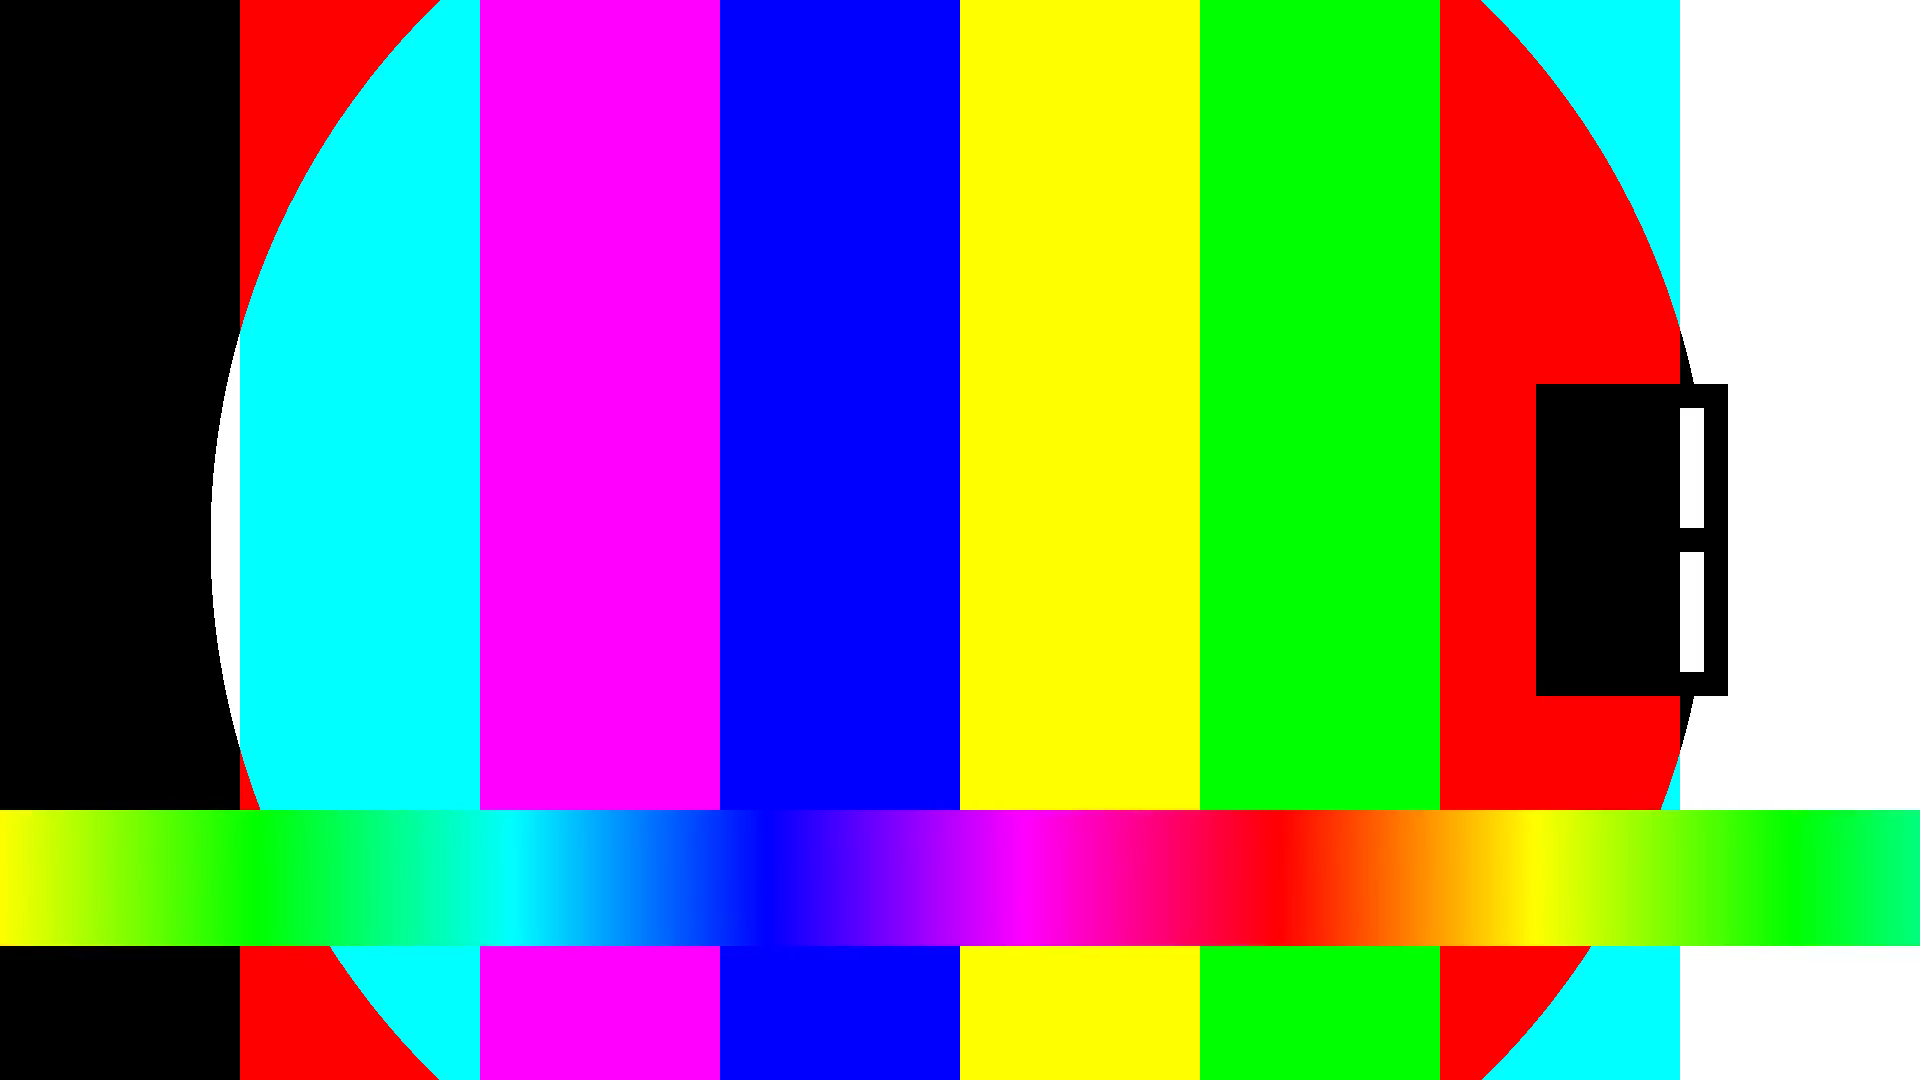
\includegraphics{poster1080p60}}{VPlayer.swf}

  \small Performance check: 60\,fps on iPad and projector while inking.
\end{frame}

\begin{frame}{3. Two embedded videos on one slide}
  \centering
  \includemedia[
    width=0.45\linewidth,height=0.253125\linewidth,
    activate=pageopen,
    addresource=clip720p30.mp4,
    flashvars={source=clip720p30.mp4&autoPlay=true&loop=true}
  ]{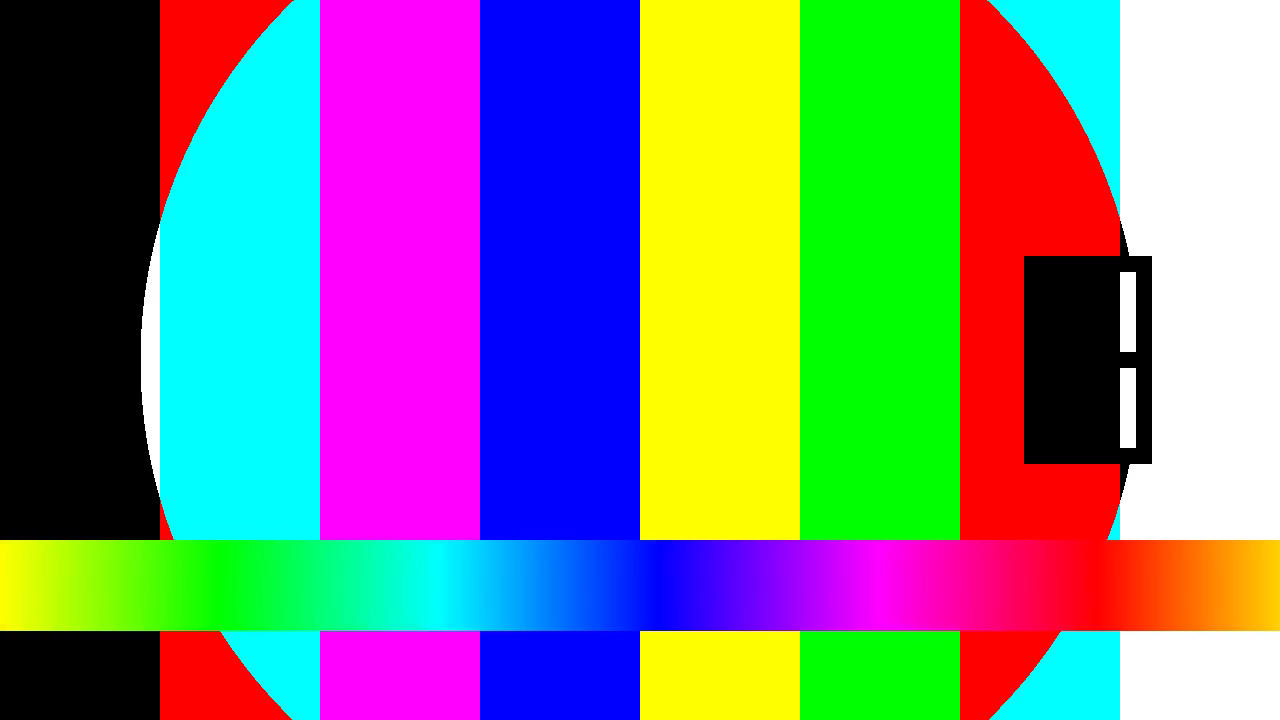
\includegraphics{poster720p30}}{VPlayer.swf}\hfill
  \includemedia[
    width=0.45\linewidth,height=0.253125\linewidth,
    activate=onclick,
    addresource=clip1080p60.mp4,
    flashvars={source=clip1080p60.mp4}
  ]{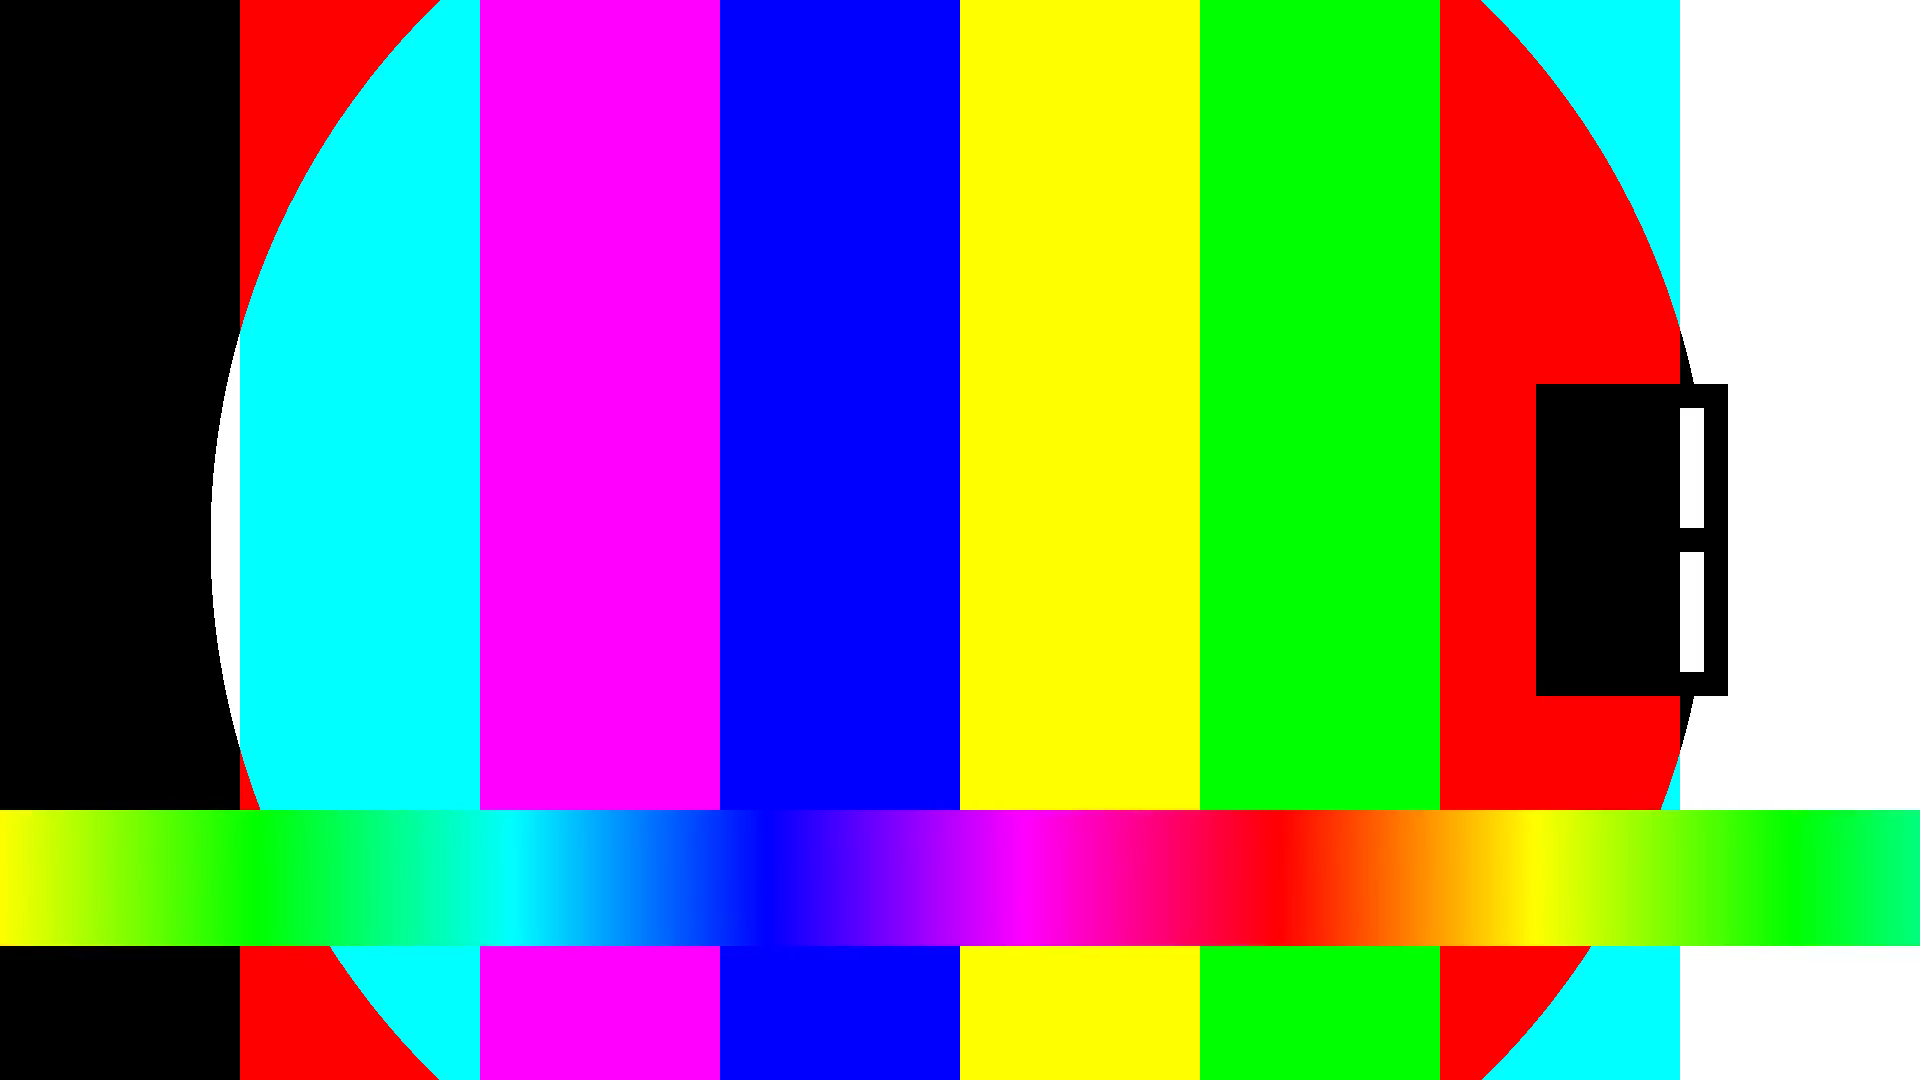
\includegraphics{poster1080p60}}{VPlayer.swf}
\end{frame}

\begin{frame}{4. \textbackslash movie: linked file (needs folder access)}
  \centering
  \movie[width=0.75\linewidth,height=0.421875\linewidth,autostart,loop]
    {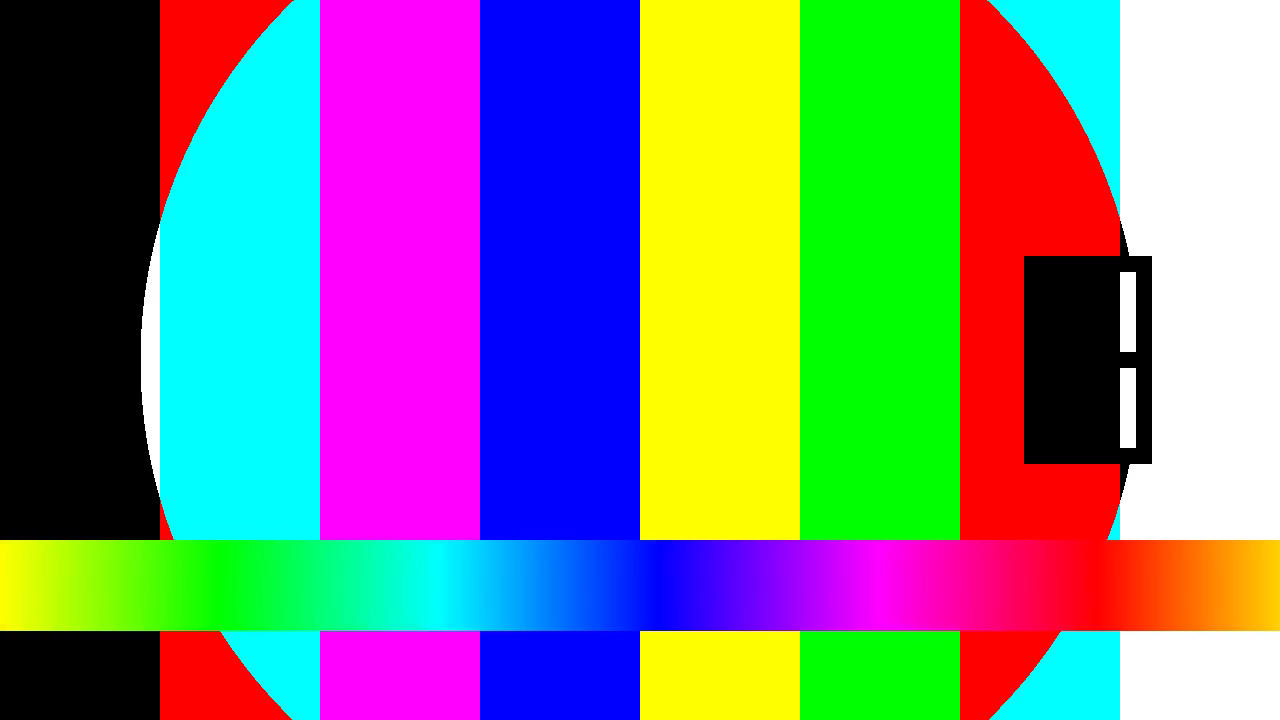
\includegraphics[width=0.75\linewidth]{poster720p30}}{clip720p30.mp4}

  \small File lives next to the PDF, not inside it.
\end{frame}

\begin{frame}{5. animate: 24 frames @ 12 fps, loop}
  \centering
  \begin{animateinline}[autoplay,loop,controls]{12}
    \multiframe{24}{rAng=0+15}{%
      \begin{tikzpicture}
        \useasboundingbox (-2.4,-2.4) rectangle (2.4,2.4);
        \draw[thick] (0,0) circle (2);
        \fill[red] (\rAng:2) circle (0.25);
        \draw[->,very thick,blue] (0,0) -- (\rAng:1.7);
        \node at (0,-1) {\rAng$^\circ$};
      \end{tikzpicture}%
    }
  \end{animateinline}
\end{frame}

\begin{frame}{5b. animate: 8 fps, play once, tap to start}
  \centering
  \begin{animateinline}{8}
    \multiframe{16}{iN=1+1}{%
      \begin{tikzpicture}
        \useasboundingbox (0,0) rectangle (8,2);
        \fill[green!60!black] (0,0.5) rectangle (\iN*0.5,1.5);
        \draw (0,0.5) rectangle (8,1.5);
        \node at (4,1.8) {frame \iN/16};
      \end{tikzpicture}%
    }
  \end{animateinline}
\end{frame}

\begin{frame}{6. Overlays (\textbackslash pause)}
  \begin{itemize}
    \item First point \pause
    \item Second point \pause
    \item Third point: ink stays across all steps
  \end{itemize}
\end{frame}

\begin{frame}{7. Vector-heavy slide (render speed)}
  \centering
  \begin{tikzpicture}
    \begin{axis}[width=0.9\linewidth,height=0.6\textheight,grid=both]
      \addplot[blue,samples=2000,domain=0:20] {sin(deg(x))*exp(-x/10)};
      \addplot[red,only marks,mark size=0.6pt,samples=1500,domain=0:20] {cos(deg(3*x))*0.5 + rand*0.1};
    \end{axis}
  \end{tikzpicture}
\end{frame}

\begin{frame}[label=links]{8. Hyperlinks}
  \hyperlink{target}{\beamergotobutton{Jump to slide 9}}\quad
  \hyperlink{media9first}{\beamergotobutton{Back to media9}}
\end{frame}

\begin{frame}[label=target]{9. Link target / blank ink slide}
  Plain slide for pen, highlighter, eraser and undo tests.
  \hyperlink{links}{\beamerreturnbutton{Back}}
\end{frame}

\end{document}
